% Created by tikzDevice version 0.12.6 on 2024-04-18 18:47:23
% !TEX encoding = UTF-8 Unicode
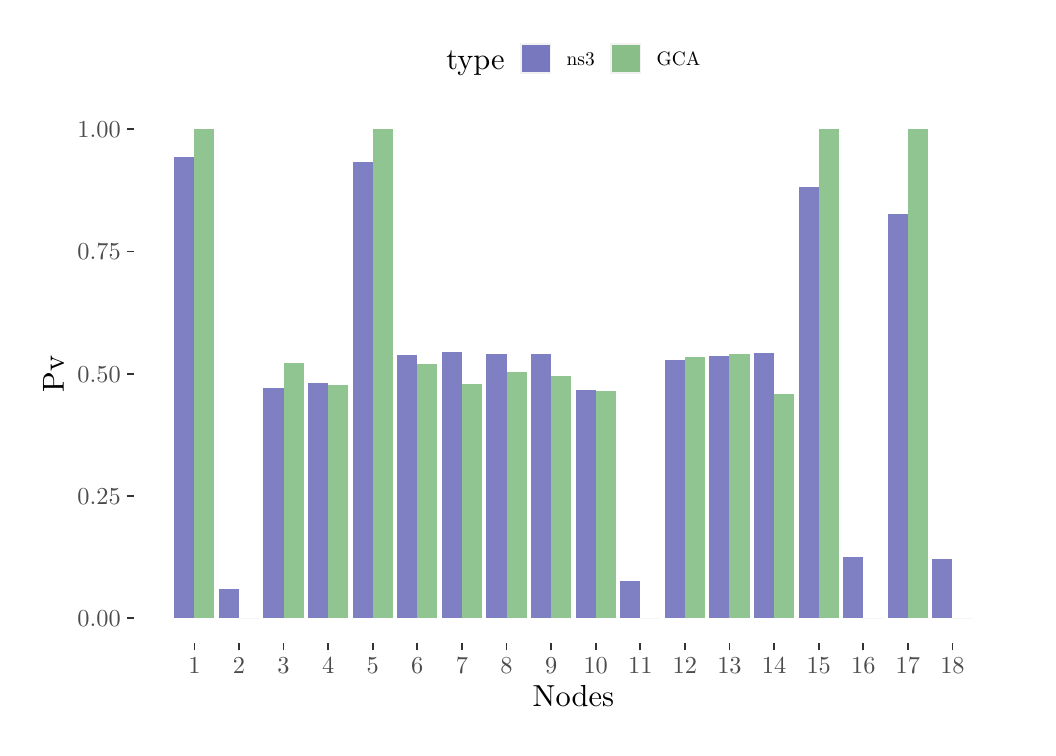
\begin{tikzpicture}[x=1pt,y=1pt]
\definecolor{fillColor}{RGB}{255,255,255}
\path[use as bounding box,fill=fillColor,fill opacity=0.00] (0,0) rectangle (361.35,252.94);
\begin{scope}
\path[clip] (  0.00,  0.00) rectangle (361.35,252.94);
\definecolor{drawColor}{RGB}{255,255,255}
\definecolor{fillColor}{RGB}{255,255,255}

\path[draw=drawColor,line width= 0.6pt,line join=round,line cap=round,fill=fillColor] (  0.00,  0.00) rectangle (361.35,252.94);
\end{scope}
\begin{scope}
\path[clip] ( 38.56, 30.69) rectangle (355.85,225.06);
\definecolor{fillColor}{RGB}{255,255,255}

\path[fill=fillColor] ( 38.56, 30.69) rectangle (355.85,225.06);
\definecolor{fillColor}{RGB}{0,0,139}

\path[fill=fillColor,fill opacity=0.50] ( 52.98, 39.52) rectangle ( 60.23,206.14);
\definecolor{fillColor}{RGB}{34,139,34}

\path[fill=fillColor,fill opacity=0.50] ( 60.23, 39.52) rectangle ( 67.48,216.23);

\path[fill=fillColor,fill opacity=0.50] ( 76.34, 39.52) rectangle ( 83.60, 39.52);
\definecolor{fillColor}{RGB}{0,0,139}

\path[fill=fillColor,fill opacity=0.50] ( 69.09, 39.52) rectangle ( 76.34, 50.07);

\path[fill=fillColor,fill opacity=0.50] ( 85.21, 39.52) rectangle ( 92.46,122.68);
\definecolor{fillColor}{RGB}{34,139,34}

\path[fill=fillColor,fill opacity=0.50] ( 92.46, 39.52) rectangle ( 99.71,131.76);

\path[fill=fillColor,fill opacity=0.50] (108.57, 39.52) rectangle (115.82,123.81);
\definecolor{fillColor}{RGB}{0,0,139}

\path[fill=fillColor,fill opacity=0.50] (101.32, 39.52) rectangle (108.57,124.72);

\path[fill=fillColor,fill opacity=0.50] (117.44, 39.52) rectangle (124.69,204.37);
\definecolor{fillColor}{RGB}{34,139,34}

\path[fill=fillColor,fill opacity=0.50] (124.69, 39.52) rectangle (131.94,216.23);

\path[fill=fillColor,fill opacity=0.50] (140.80, 39.52) rectangle (148.05,131.41);
\definecolor{fillColor}{RGB}{0,0,139}

\path[fill=fillColor,fill opacity=0.50] (133.55, 39.52) rectangle (140.80,134.76);
\definecolor{fillColor}{RGB}{34,139,34}

\path[fill=fillColor,fill opacity=0.50] (156.92, 39.52) rectangle (164.17,124.16);
\definecolor{fillColor}{RGB}{0,0,139}

\path[fill=fillColor,fill opacity=0.50] (149.66, 39.52) rectangle (156.92,135.76);
\definecolor{fillColor}{RGB}{34,139,34}

\path[fill=fillColor,fill opacity=0.50] (173.03, 39.52) rectangle (180.28,128.58);
\definecolor{fillColor}{RGB}{0,0,139}

\path[fill=fillColor,fill opacity=0.50] (165.78, 39.52) rectangle (173.03,134.94);
\definecolor{fillColor}{RGB}{34,139,34}

\path[fill=fillColor,fill opacity=0.50] (189.15, 39.52) rectangle (196.40,127.17);
\definecolor{fillColor}{RGB}{0,0,139}

\path[fill=fillColor,fill opacity=0.50] (181.89, 39.52) rectangle (189.15,134.95);
\definecolor{fillColor}{RGB}{34,139,34}

\path[fill=fillColor,fill opacity=0.50] (205.26, 39.52) rectangle (212.51,121.51);
\definecolor{fillColor}{RGB}{0,0,139}

\path[fill=fillColor,fill opacity=0.50] (198.01, 39.52) rectangle (205.26,121.93);
\definecolor{fillColor}{RGB}{34,139,34}

\path[fill=fillColor,fill opacity=0.50] (221.37, 39.52) rectangle (228.63, 39.52);
\definecolor{fillColor}{RGB}{0,0,139}

\path[fill=fillColor,fill opacity=0.50] (214.12, 39.52) rectangle (221.37, 53.05);

\path[fill=fillColor,fill opacity=0.50] (230.24, 39.52) rectangle (237.49,132.90);
\definecolor{fillColor}{RGB}{34,139,34}

\path[fill=fillColor,fill opacity=0.50] (237.49, 39.52) rectangle (244.74,134.06);
\definecolor{fillColor}{RGB}{0,0,139}

\path[fill=fillColor,fill opacity=0.50] (246.35, 39.52) rectangle (253.60,134.40);
\definecolor{fillColor}{RGB}{34,139,34}

\path[fill=fillColor,fill opacity=0.50] (253.60, 39.52) rectangle (260.85,135.12);

\path[fill=fillColor,fill opacity=0.50] (269.72, 39.52) rectangle (276.97,120.45);
\definecolor{fillColor}{RGB}{0,0,139}

\path[fill=fillColor,fill opacity=0.50] (262.47, 39.52) rectangle (269.72,135.24);

\path[fill=fillColor,fill opacity=0.50] (278.58, 39.52) rectangle (285.83,195.41);
\definecolor{fillColor}{RGB}{34,139,34}

\path[fill=fillColor,fill opacity=0.50] (285.83, 39.52) rectangle (293.08,216.23);

\path[fill=fillColor,fill opacity=0.50] (301.95, 39.52) rectangle (309.20, 39.52);
\definecolor{fillColor}{RGB}{0,0,139}

\path[fill=fillColor,fill opacity=0.50] (294.70, 39.52) rectangle (301.95, 61.83);

\path[fill=fillColor,fill opacity=0.50] (310.81, 39.52) rectangle (318.06,185.75);
\definecolor{fillColor}{RGB}{34,139,34}

\path[fill=fillColor,fill opacity=0.50] (318.06, 39.52) rectangle (325.31,216.23);

\path[fill=fillColor,fill opacity=0.50] (334.18, 39.52) rectangle (341.43, 39.52);
\definecolor{fillColor}{RGB}{0,0,139}

\path[fill=fillColor,fill opacity=0.50] (326.92, 39.52) rectangle (334.18, 61.08);
\end{scope}
\begin{scope}
\path[clip] (  0.00,  0.00) rectangle (361.35,252.94);
\definecolor{drawColor}{gray}{0.30}

\node[text=drawColor,anchor=base east,inner sep=0pt, outer sep=0pt, scale=  0.88] at ( 33.61, 36.49) {0.00};

\node[text=drawColor,anchor=base east,inner sep=0pt, outer sep=0pt, scale=  0.88] at ( 33.61, 80.67) {0.25};

\node[text=drawColor,anchor=base east,inner sep=0pt, outer sep=0pt, scale=  0.88] at ( 33.61,124.84) {0.50};

\node[text=drawColor,anchor=base east,inner sep=0pt, outer sep=0pt, scale=  0.88] at ( 33.61,169.02) {0.75};

\node[text=drawColor,anchor=base east,inner sep=0pt, outer sep=0pt, scale=  0.88] at ( 33.61,213.20) {1.00};
\end{scope}
\begin{scope}
\path[clip] (  0.00,  0.00) rectangle (361.35,252.94);
\definecolor{drawColor}{gray}{0.20}

\path[draw=drawColor,line width= 0.6pt,line join=round] ( 35.81, 39.52) --
	( 38.56, 39.52);

\path[draw=drawColor,line width= 0.6pt,line join=round] ( 35.81, 83.70) --
	( 38.56, 83.70);

\path[draw=drawColor,line width= 0.6pt,line join=round] ( 35.81,127.87) --
	( 38.56,127.87);

\path[draw=drawColor,line width= 0.6pt,line join=round] ( 35.81,172.05) --
	( 38.56,172.05);

\path[draw=drawColor,line width= 0.6pt,line join=round] ( 35.81,216.23) --
	( 38.56,216.23);
\end{scope}
\begin{scope}
\path[clip] (  0.00,  0.00) rectangle (361.35,252.94);
\definecolor{drawColor}{gray}{0.20}

\path[draw=drawColor,line width= 0.6pt,line join=round] ( 60.23, 27.94) --
	( 60.23, 30.69);

\path[draw=drawColor,line width= 0.6pt,line join=round] ( 76.34, 27.94) --
	( 76.34, 30.69);

\path[draw=drawColor,line width= 0.6pt,line join=round] ( 92.46, 27.94) --
	( 92.46, 30.69);

\path[draw=drawColor,line width= 0.6pt,line join=round] (108.57, 27.94) --
	(108.57, 30.69);

\path[draw=drawColor,line width= 0.6pt,line join=round] (124.69, 27.94) --
	(124.69, 30.69);

\path[draw=drawColor,line width= 0.6pt,line join=round] (140.80, 27.94) --
	(140.80, 30.69);

\path[draw=drawColor,line width= 0.6pt,line join=round] (156.92, 27.94) --
	(156.92, 30.69);

\path[draw=drawColor,line width= 0.6pt,line join=round] (173.03, 27.94) --
	(173.03, 30.69);

\path[draw=drawColor,line width= 0.6pt,line join=round] (189.15, 27.94) --
	(189.15, 30.69);

\path[draw=drawColor,line width= 0.6pt,line join=round] (205.26, 27.94) --
	(205.26, 30.69);

\path[draw=drawColor,line width= 0.6pt,line join=round] (221.37, 27.94) --
	(221.37, 30.69);

\path[draw=drawColor,line width= 0.6pt,line join=round] (237.49, 27.94) --
	(237.49, 30.69);

\path[draw=drawColor,line width= 0.6pt,line join=round] (253.60, 27.94) --
	(253.60, 30.69);

\path[draw=drawColor,line width= 0.6pt,line join=round] (269.72, 27.94) --
	(269.72, 30.69);

\path[draw=drawColor,line width= 0.6pt,line join=round] (285.83, 27.94) --
	(285.83, 30.69);

\path[draw=drawColor,line width= 0.6pt,line join=round] (301.95, 27.94) --
	(301.95, 30.69);

\path[draw=drawColor,line width= 0.6pt,line join=round] (318.06, 27.94) --
	(318.06, 30.69);

\path[draw=drawColor,line width= 0.6pt,line join=round] (334.18, 27.94) --
	(334.18, 30.69);
\end{scope}
\begin{scope}
\path[clip] (  0.00,  0.00) rectangle (361.35,252.94);
\definecolor{drawColor}{gray}{0.30}

\node[text=drawColor,anchor=base,inner sep=0pt, outer sep=0pt, scale=  0.88] at ( 60.23, 19.68) {1};

\node[text=drawColor,anchor=base,inner sep=0pt, outer sep=0pt, scale=  0.88] at ( 76.34, 19.68) {2};

\node[text=drawColor,anchor=base,inner sep=0pt, outer sep=0pt, scale=  0.88] at ( 92.46, 19.68) {3};

\node[text=drawColor,anchor=base,inner sep=0pt, outer sep=0pt, scale=  0.88] at (108.57, 19.68) {4};

\node[text=drawColor,anchor=base,inner sep=0pt, outer sep=0pt, scale=  0.88] at (124.69, 19.68) {5};

\node[text=drawColor,anchor=base,inner sep=0pt, outer sep=0pt, scale=  0.88] at (140.80, 19.68) {6};

\node[text=drawColor,anchor=base,inner sep=0pt, outer sep=0pt, scale=  0.88] at (156.92, 19.68) {7};

\node[text=drawColor,anchor=base,inner sep=0pt, outer sep=0pt, scale=  0.88] at (173.03, 19.68) {8};

\node[text=drawColor,anchor=base,inner sep=0pt, outer sep=0pt, scale=  0.88] at (189.15, 19.68) {9};

\node[text=drawColor,anchor=base,inner sep=0pt, outer sep=0pt, scale=  0.88] at (205.26, 19.68) {10};

\node[text=drawColor,anchor=base,inner sep=0pt, outer sep=0pt, scale=  0.88] at (221.37, 19.68) {11};

\node[text=drawColor,anchor=base,inner sep=0pt, outer sep=0pt, scale=  0.88] at (237.49, 19.68) {12};

\node[text=drawColor,anchor=base,inner sep=0pt, outer sep=0pt, scale=  0.88] at (253.60, 19.68) {13};

\node[text=drawColor,anchor=base,inner sep=0pt, outer sep=0pt, scale=  0.88] at (269.72, 19.68) {14};

\node[text=drawColor,anchor=base,inner sep=0pt, outer sep=0pt, scale=  0.88] at (285.83, 19.68) {15};

\node[text=drawColor,anchor=base,inner sep=0pt, outer sep=0pt, scale=  0.88] at (301.95, 19.68) {16};

\node[text=drawColor,anchor=base,inner sep=0pt, outer sep=0pt, scale=  0.88] at (318.06, 19.68) {17};

\node[text=drawColor,anchor=base,inner sep=0pt, outer sep=0pt, scale=  0.88] at (334.18, 19.68) {18};
\end{scope}
\begin{scope}
\path[clip] (  0.00,  0.00) rectangle (361.35,252.94);
\definecolor{drawColor}{RGB}{0,0,0}

\node[text=drawColor,anchor=base,inner sep=0pt, outer sep=0pt, scale=  1.10] at (197.20,  7.64) {Nodes};
\end{scope}
\begin{scope}
\path[clip] (  0.00,  0.00) rectangle (361.35,252.94);
\definecolor{drawColor}{RGB}{0,0,0}

\node[text=drawColor,rotate= 90.00,anchor=base,inner sep=0pt, outer sep=0pt, scale=  1.10] at ( 13.08,127.87) {Pv};
\end{scope}
\begin{scope}
\path[clip] (  0.00,  0.00) rectangle (361.35,252.94);
\definecolor{fillColor}{RGB}{255,255,255}

\path[fill=fillColor] (151.31,236.06) rectangle (243.09,247.45);
\end{scope}
\begin{scope}
\path[clip] (  0.00,  0.00) rectangle (361.35,252.94);
\definecolor{drawColor}{RGB}{0,0,0}

\node[text=drawColor,anchor=base west,inner sep=0pt, outer sep=0pt, scale=  1.10] at (151.31,237.97) {type};
\end{scope}
\begin{scope}
\path[clip] (  0.00,  0.00) rectangle (361.35,252.94);
\definecolor{fillColor}{gray}{0.95}

\path[fill=fillColor] (177.89,236.06) rectangle (189.27,247.45);
\end{scope}
\begin{scope}
\path[clip] (  0.00,  0.00) rectangle (361.35,252.94);
\definecolor{fillColor}{RGB}{0,0,139}

\path[fill=fillColor,fill opacity=0.50] (178.60,236.78) rectangle (188.56,246.73);
\end{scope}
\begin{scope}
\path[clip] (  0.00,  0.00) rectangle (361.35,252.94);
\definecolor{fillColor}{gray}{0.95}

\path[fill=fillColor] (210.42,236.06) rectangle (221.80,247.45);
\end{scope}
\begin{scope}
\path[clip] (  0.00,  0.00) rectangle (361.35,252.94);
\definecolor{fillColor}{RGB}{34,139,34}

\path[fill=fillColor,fill opacity=0.50] (211.13,236.78) rectangle (221.09,246.73);
\end{scope}
\begin{scope}
\path[clip] (  0.00,  0.00) rectangle (361.35,252.94);
\definecolor{drawColor}{RGB}{0,0,0}

\node[text=drawColor,anchor=base west,inner sep=0pt, outer sep=0pt, scale=  0.70] at (194.77,239.34) {ns3};
\end{scope}
\begin{scope}
\path[clip] (  0.00,  0.00) rectangle (361.35,252.94);
\definecolor{drawColor}{RGB}{0,0,0}

\node[text=drawColor,anchor=base west,inner sep=0pt, outer sep=0pt, scale=  0.70] at (227.30,239.34) {GCA};
\end{scope}
\end{tikzpicture}
